\begin{figure}[H]
  \centering
  \begin{subfigure}[t]{0.6\textwidth}
      \begin{algorithm}[H]
        $N \gets $ $number$ $of$ $children$ $of$ $the$ $node$\;
        $i \gets 0$\;
        \While{$i < N$}{
            $childStatus$ $\gets$ $tick(child[i])$\\    
        {\If{childStatus == running or\\
              childStatus == failure }{
              \textbf{return} $childStatus$
            }
          }
        }
        \textbf{return} $childStatus$
    \end{algorithm}
    
      \caption{Pseudo code for sequence node}\label{alg:seq}
      % \caption{Lorem ipsum}
  \end{subfigure}%
  ~ 
  \begin{subfigure}[t]{0.3\textwidth}
      \centering
      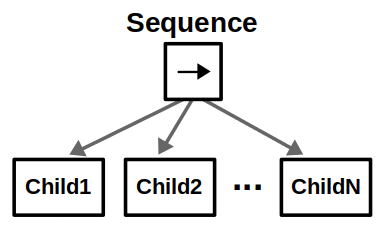
\includegraphics{figs/bt_sequence_node.png}
      \caption{Graphical representation of the node}
      \label{fig:seq}
  \end{subfigure}
  \caption{Caption place holder}
\end{figure}